\section{Simulado 1}

\num{1}

\textbf{Direito de ter direitos}

\begin{quote}
Cidadania -- uma palavra usada com frequência, mas que poucos entendem o
que significa -- quer dizer, em essência, a garantia por lei de viver
dignamente. É o direito de expressar as próprias ideias; de votar em
quem quiser sem nenhum tipo de constrangimento; de processar um médico
ou hospital por negligência ou imperícia; de devolver um produto
estragado e receber o dinheiro de volta; {[}...{]}

O direito de ter direitos foi uma conquista árdua da humanidade. No
Brasil, por exemplo, demorou muito tempo para que as pessoas tivessem o
direito de votar e escolher seus governantes. {[}...{]}
\end{quote}

\fonte{DIMENSTEIN, Gilberto. \emph{O cidadão de papel}: a infância, a
adolescência e os Direitos Humanos no Brasil. 24.ed. São Paulo: Ática,
2012.}

No texto, o trecho isolado por travessões pode ser interpretado como

\begin{escolha}
\item uma crítica.

\item um conselho.

\item uma dedução.

\item uma suposição.
\end{escolha}

\num{2}

\begin{figure}
\centering
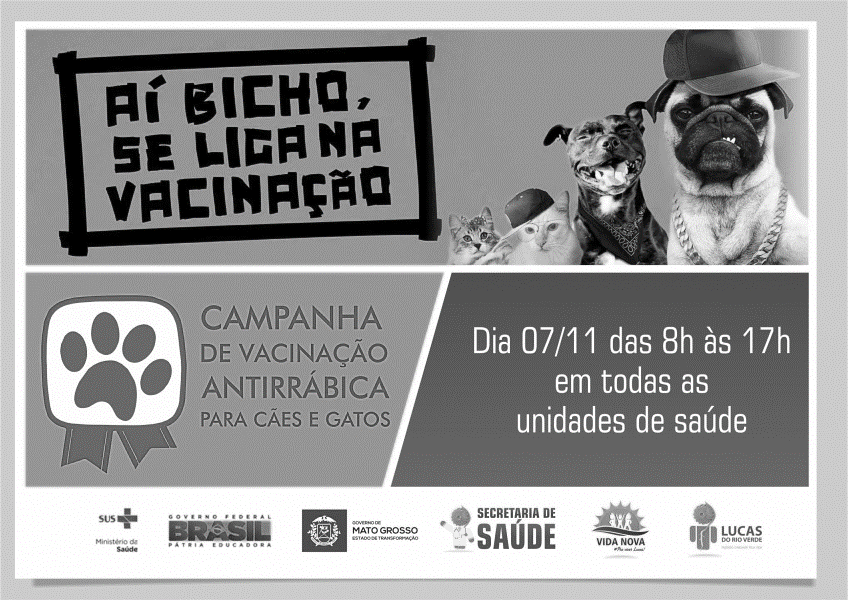
\includegraphics[width=4.03125in,height=2.85231in]{./imgSAEB_8_POR/media/image28.png}
\caption{Uma imagem contendo Código QR Descrição gerada automaticamente}
\end{figure}

\fonte{Disponível em: \url{https://lucasdorioverde.mt.gov.br/site/noticias/campanha-de-vacinacao-antirrabica-sera-realizada-neste-sabado-07-5018\gallery.}
Acesso em: 10 fev. 2023.}

A relação entre a imagem e a linguagem verbal é evidenciada, no texto da
campanha, pela presença de

\begin{escolha}
\item frases curtas.

\item frases nominais.

\item nomes de animais.

\item gírias de interação.
\end{escolha}

\num{3}

\begin{quote}
Pescadores e caçadores são sempre os heróis de suas histórias {[}...{]}.
Quem quiser acreditar neste causo, aqui relatado, que acredite! Não sou
pescador, não sou caçador, sou apenas ouvinte. Ao ouvir este causo,
achei-o interessante e o escrevi, conforme segue nas linhas abaixo...

O causo se deu no Norte de Minas Gerais, numa cidadezinha rancheira,
onde o povo completava a sua alimentação com a pesca e com a caça.

Dizem que nessa cidadezinha existia um grande caçador, qual habilidade
queria passar ao filho primogênito de 15 anos. Ele procurava um modo de
parafrasear a famosa premissa popular: ``filho de peixe, peixinho é'',
tomando-a para ele como ``filho de caçador, caçadorzinho é''. {[}...{]}
\end{quote}

\fonte{RODRIGUES JÚNIOR, Francisco. \emph{Causos de Minas} -- Literatura:
memória, identidade e cultura mineira. Selo editorial: Independently
published, 2014 (fragmento).}

Em qual trecho texto o narrador se exime do compromisso com a veracidade
do causo que ele conta?

\begin{escolha}
\item ``Não sou pescador, não sou caçador, sou apenas ouvinte.''

\item ``Quem quiser acreditar neste causo, aqui relatado, que acredite!''

\item ``Ele procurava um modo de parafrasear a famosa premissa popular:''

\item ``O causo se deu no Norte de Minas Gerais, numa cidadezinha rancheira
{[}...{]}.''
\end{escolha}

\textbf{Texto para as questões 4 e 5.}

\begin{quote}
Fernando foi passar as férias na casa de Pedro, um amigo que mora há
muito tempo em outro
estado. Enquanto aproveitam a praia, eles conversam:

-- Nossa, que fome! Me dá uma bolacha aí!

-- Não tenho bolacha.

-- Então o que é isso que você tá comendo?

-- Biscoito.

-- Ah, tanto faz, o importante é matar a fome!

-- Tá bem, eu dou, mas você quer biscoito ou bolacha?

-- Não importa, tô com fome!
\end{quote}

\fonte{Elaborado pelo autor.}

\num{4}

No diálogo, o fato de os amigos viverem em regiões diferentes faz com
que eles

\begin{escolha}
\item tenham opiniões diferentes sobre o sabor do alimento.

\item prefiram o biscoito ou a bolacha a qualquer outro lanche.

\item usem palavras diferentes para nomear o mesmo alimento.

\item discutam sobre a diferença de sabor entre o biscoito e a bolacha.
\end{escolha}

\num{5}

O traço de humor do texto reside

\begin{escolha}
\item na indiferença de um dos amigos ao aceitar qualquer um dos lanches.

\item no pedido de um dos amigos ao querer comida num ambiente de praia.

\item no uso de abreviações de palavras numa situação que exigia
formalidade.

\item na atitude de um dos amigos ao fingir não conhecer a palavra usada
pelo colega.
\end{escolha}

\num{6}

\begin{longtable}[]{@{}ll@{}}
\toprule
\endhead
\begin{minipage}[t]{0.46\columnwidth}\raggedright
(./imgSAEB\_8\_POR/media/image29.png)\{width=``2.2083333333333335in''
height=``2.2083333333333335in''\}

\fonte{Disponível em: \url{https://www.ibiting a.sp.gov.br/noticias/saude/vacina-contra-gripe-comeca-segunda-fe ira-em-idosos-acima-de-80-anos}.
Acesso em: 10 fev. 2023.}

\strut
\end{minipage} & \begin{minipage}[t]{0.46\columnwidth}\raggedright
\begin{quote}
{[}Uma imagem contendo texto, placar, grama, placa Descrição gerada
automaticamente{]} (./imgSAEB\_8\_POR/media/image30.p
ng)\{width=``2.7083333333333335in'' height=``2.2029101049868767in''\}
\end{quote}

\fonte{Disponível em: \url{https://www.parac uru.ce.gov.br/informa.php?id=64}.
Acesso em: 10 fev. 2023.}

\strut
\end{minipage}\tabularnewline
\bottomrule
\end{longtable}

Os dois textos têm em comum o fato de abordarem o mesmo assunto, mas sua
estratégia argumentativa se diferencia condicionada pelo

\begin{escolha}
\item assunto.

\item público-alvo.

\item meio de circulação.

\item objetivo comunicativo.
\end{escolha}

\textbf{Texto para as questões 7 e 8.}

\begin{quote}
Bom, inicialmente gostaria de agradecer a presença de todos. Para mim é
uma oportunidade importante, única e emotiva também, de mostrar o meu
trabalho. Enfim, é a função da minha vida. E gostaria de agradecer o
convite feito pelos professores e artistas. Vou fazer um depoimento
sobre a minha obra, sobre o meu trabalho. É a primeira vez que apresento
a grande maioria desses eslaides. Preparei uma seleção de imagens
focando a apresentação na produção de desenho, que é tema deste
seminário. Na verdade, meu surgimento como artista deu-se como
desenhista, e é bom que eu diga de início para, desde já, dar uma
resposta para essa questão do desenho como ponte: o desenho me colocou
no mundo, me colocou em contato com a minha comunidade, com as pessoas,
com o mundo em geral. {[}...{]}
\end{quote}

\fonte{Disponível em: \url{https://seer.ufrgs.br/RevistaValise/article/download/41375/26239.}
Acesso em: 16 fev. 2023 (fragmento adaptado).}

\num{7}

O trecho é a transcrição de uma apresentação oral feita em um seminário
universitário. Nesse contexto, o autor do texto privilegia o uso da
linguagem

\begin{escolha}
\item
  coloquial, buscando interagir com as pessoas da plateia.
\item
  técnica, usando termos da área profissional em que atua.
\item
  formal, promovendo a adequação à situação comunicativa.
\item
  regional, empregando o vocabulário da região dos ouvintes.
\end{escolha}

\num{8}

O trecho ``Preparei uma seleção de imagens focando a apresentação na
produção de desenho, que é tema deste seminário'' contém o elemento
linguístico ``deste seminário'', que aponta para

\begin{escolha}
\item um elemento externo ao texto.

\item um elemento já citado no texto.

\item um elemento a ser citado no texto.

\item um elemento que pertence ao autor.
\end{escolha}

\num{9}

\begin{quote}
Trago dentro do meu coração,

Como num cofre que se não pode fechar de cheio,

Todos os lugares onde estive,

Todos os portos a que cheguei,

Todas as paisagens que vi através de janelas ou vigias,

{[}...{]}

A entrada de Singapura, manhã subindo, cor verde,

O coral das Maldivas em passagem cálida,

{[}...{]}

E o Cabo da Boa Esperança nítido ao sol da madrugada...

E a Cidade do Cabo com a Montanha da Mesa ao fundo...
\end{quote}
\fonte{
PESSOA, F. Disponível em: \url{http://www.dominiopublico.gov.br/download/texto/pe000010.pdf.}
Acesso em: 11 fev. 2023 (fragmento).}

O eu lírico expressa no poema, como tema central,

\begin{escolha}
\item a saudade da sua terra natal.

\item as lembranças das suas viagens.

\item a vontade de conhecer o mundo.

\item o gosto pelas belezas da natureza.
\end{escolha}

\num{10}

\begin{figure}
\centering

\includegraphics[width=4.21103in,height=2.86458in]{./imgSAEB_8_POR/media/image31.png}
\caption{Texto Descrição gerada automaticamente com confiança média}
\end{figure}

\fonte{Disponível em: \url{https://www.novaguarita.mt.gov.br/Noticias/Campanha-julho-amarelo-mes-de-prevencao-e-conscientizacao-contra-hepatites-virais-/-796.} Acesso em: 16 fev. 2023.}

A estratégia de persuasão empregada no texto enfatiza

\begin{escolha}
\item
  a forma de contágio da doença.
\item
  os integrantes do grupo de risco.
\item
  a ausência de sintomas da doença.
\item
  os fatores de risco para o contágio.
\end{escolha}

\num{11}

\textbf{TEXTO I}

\begin{quote}
\textbf{Estudo alerta para vacinação infantil abaixo da meta no estado
do Rio}

\emph{Prefeituras têm até 2024 para fornecer dados ao Ministério da
Saúde}

As metas de cobertura vacinal de crianças menores de cinco anos não
foram atingidas no estado do Rio de Janeiro para nenhuma das vacinas do
calendário infantil de 2022, alerta levantamento preliminar divulgado
nesta terça-feira (27) pela Fundação Oswaldo Cruz (Fiocruz).

Apesar de ser o segundo estado mais rico do país, o Rio de Janeiro
também está abaixo da cobertura média nacional de todas as vacinas, não
chegando a atingir metade do público-alvo no caso das proteções contra
poliomielite, difteria, tétano, coqueluche, hepatite B, pneumonia e
meningite bacterianas. {[}...{]}

Mesmo que alguns municípios consigam atingir as metas para algumas
vacinas com a atualização dos dados, a coordenadora do Observa Infância,
Patricia Boccolini, avaliou que o cenário geral do estado continuará
sendo de baixas coberturas. {[}...{]}

\end{quote}
\fonte{
Disponível em: \url{https://agenciabrasil.ebc.com.br/saude/noticia/2022-12/estudo-alerta-para-vacinacao-infantil-abaixo-da-meta-no-estado-do-rio.}
Acesso em: 13 fev. 2023 (fragmento).}

\textbf{TEXTO II}

\begin{figure}
\centering
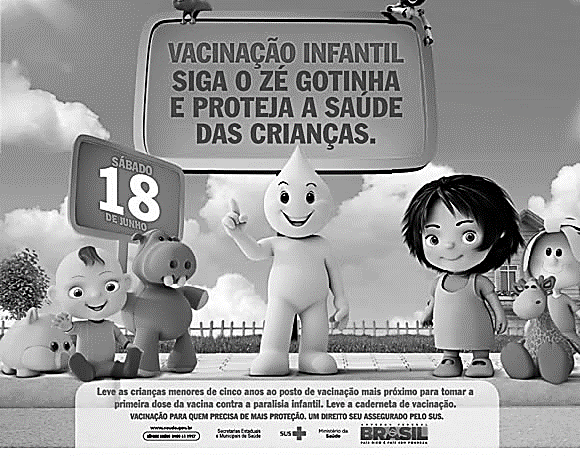
\includegraphics[width=3.15625in,height=2.48418in]{./imgSAEB_8_POR/media/image32.png}
\caption{http://2.bp.blogspot.com/-cla\_CLQDT4U/TfZ28yGeWWI/AAAAAAAAAJA/Vjwyrj1fc1A/s1600/campanha-poliomielite-2011.jpg}
\end{figure}
\fonte{
Disponível em: \url{
https://saude.es.gov.br/dia-d-da-campanha-de-vacinacao-contra-a-polio.
Acesso em: 13 fev. 2023.}}

Comparando-se os dois textos, conclui-se que o texto II cumpre, em
relação à situação noticiada no texto I, a função de

\begin{escolha}
\item apresentar o personagem Zé Gotinha e seus amigos ao público infantil.

\item convidar as crianças a seguirem as redes sociais do personagem Zé
Gotinha.

\item divulgar as campanhas de vacinação infantil do governo e atrair a
população.

\item entreter o público infantil com ilustrações sobre vacinação adequadas
à faixa etária.
\end{escolha}

\num{12}

\textbf{TEXTO I}

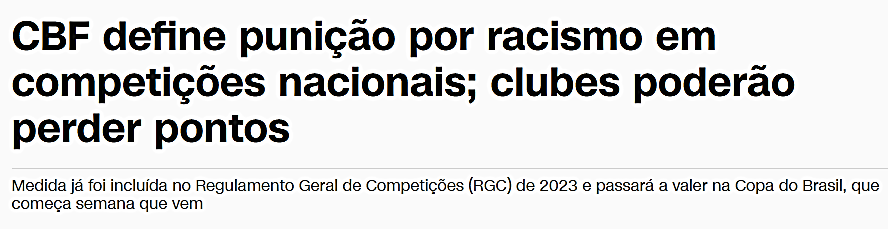
\includegraphics[width=5.34306in,height=1.37786in]{./imgSAEB_8_POR/media/image33.png}

\fonte{Disponível
em: \url{https://www.cnnbrasil.com.br/esporte/cbf-define-punicao-por-racismo-em-competicoes-nacionais-clubes-poderao-perder-pontos/}.
Acesso em: 17 fev. 2023 (fragmento).}

\textbf{TEXTO II}

\begin{figure}
\centering
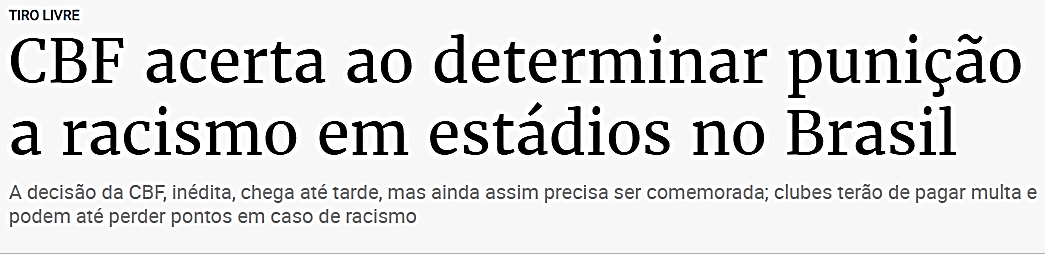
\includegraphics[width=5.47847in,height=1.37348in]{./imgSAEB_8_POR/media/image34.png}
\caption{Interface gráfica do usuário, Texto, Aplicativo Descrição
gerada automaticamente}
\end{figure}

\fonte{
Disponível em: \url{https://www.em.com.br/app/colunistas/kelen-cristina/2023/02/16/interna\kelen\cristina,1458525/cbf-acerta-ao-determinar-punicao-a-racismo-em-estadios-no-brasil.shtml.}
Acesso em: 17 fev. 2023 (fragmento).}

Ao se deparar com os fragmentos de texto I e II, sobre o mesmo assunto,
o leitor pode prever que a finalidade deles é, respectivamente,

\begin{escolha}
\item informar e opinar.

\item criticar e informar.

\item opinar e denunciar.

\item reivindicar e conscientizar.
\end{escolha}

\num{13}

\begin{figure}
\centering
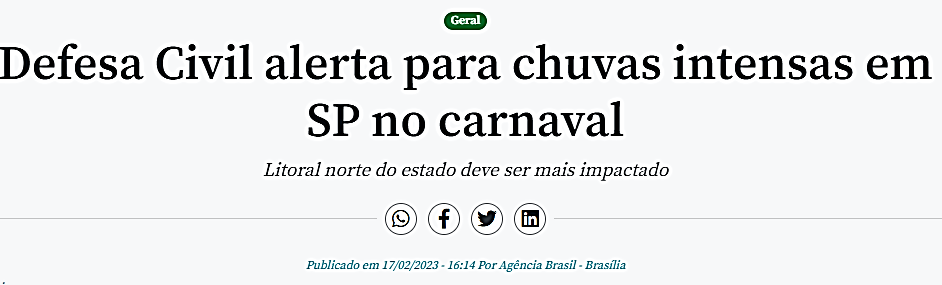
\includegraphics[width=5.90556in,height=1.78681in]{./imgSAEB_8_POR/media/image4.png}
\caption{Interface gráfica do usuário, Texto, Aplicativo, chat ou
mensagem de texto, Email Descrição gerada automaticamente}
\end{figure}

\begin{quote}
O carnaval em São Paulo terá chuvas intensas, segundo alerta da Defesa
Civil Estadual. A previsão meteorológica é que o volume alcance de 80
milímetros a 250 milímetros até domingo (19). O litoral norte do estado
deve ser o mais impactado. A Baixada Santista, Serra da Mantiqueira,
Vale do Ribeira e Itapeva podem ter até 150 milímetros de chuvas. Com o
solo já encharcado, há risco de deslizamentos em regiões de encosta.
\end{quote}

\fonte{
Disponível em: \url{https://agenciabrasil.ebc.com.br/geral/noticia/2023-02/defesa-civil-alerta-para-chuvas-intensas-no-carnaval-em-sao-paulo.}
Acesso em: 17 fev. 2023 (fragmento).}

A finalidade do texto é informar a previsão do tempo. As formas verbais
``alcance'', ``deve ser'' e ``podem ter'' estão empregadas nos tempos e
modos verbais adequados para

\begin{escolha}
\item quantificar o volume de chuvas que é esperado para o período de
carnaval.

\item recomendar cautela e atenção à população que vive nas regiões
mencionadas.

\item ressaltar o alerta de chuvas intensas que foi emitido pela Defesa
Civil Estadual.

\item exprimir a ideia de possibilidade e hipótese do que pode acontecer
com o clima.
\end{escolha}

\textbf{Texto para as questões 14 e 15.}

\begin{quote}
-- Gosto muito de ouvir você, Olívia. Sei que vou me esquecer... Espero
que você não se importe de repetir sua história outras vezes. Você se
importa?

-- Não.

-- Ouvirei sempre como se fosse a primeira vez. Isso é o que posso
prometer. E não é pouco, viu? A primeira vez tem sempre os melhores
ouvidos. Quando ouvi ``Erbarme dich'', de Bach, pela primeira vez...
Você conhece essa música?

-- Acho que não... talvez.
\end{quote}
\fonte{MADEIRA, Carla. \emph{A natureza da mordida.} 1.ed. Rio de Janeiro:
Record, 2022 (fragmento).}

\num{14}

No diálogo, a personagem é interpelada duas vezes. Em relação à segunda
pergunta que lhe é feita, sua resposta expressa

\begin{escolha}
\item hesitação.

\item desinteresse.

\item constrangimento.

\item desconhecimento.
\end{escolha}


\num{15}

A figura de linguagem empregada em ``A primeira vez tem sempre os
melhores ouvidos'' introduz a intenção de

\begin{escolha}
\item expressar a opinião da locutora em relação à melodia de Bach.

\item recomendar a apreciação da melodia ``Erbarme dich'', de Bach.

\item valorizar o esforço da personagem Olívia de recontar sua história.

\item desculpar-se pelo esquecimento da história de vida contada antes.
\end{escolha}


\_\_\_\_\_\_\_\_\_\_\_\_\_\_\_\_\_\_\_\_\_\_\_\_\_\_\_\_\_\_\_\_\_\_\_\_\_\_\_\_\_\_\_\_\_\_\_\_\_\_\_\_\_\_\_\_\_\_\_\_\_\_\_\_\_\_\_\_\_\_

\section{Simulado 2}

\num{1}

\textbf{Mudança}

\begin{quote}
Levantei as 6 hóras preparando as roupas, fazendo trouxas para zarpar da
favela. Fiz o café e fui comprar pão, pedi ao Chico para atender-me logo
porque eu ia mudar.

-- Para onde?

-- Vou ressidir em Osasco.

Ele serviu logo, paguei e sai correndo.

Estava preparando os trastes quando chegou o senhor Paulino de Moura
dono da livraria Boulevard. Vêio convidar-me para eu ir na sua livraria
autografar os meus livros.

Eu disse-lhe que irei depois que agêitar a vida dos meus filhos porque,
quando eu os deixo na favela os favelados maltrata-os. {[}...{]}
\end{quote}

\fonte{JESUS, Carolina Maria de. \emph{Casa de alvenaria, volume 1}: Osasco.
1.ed.
São Paulo: Companhia das Letras, 2021 (fragmento).}

O texto deve ser considerado um exemplo de

\begin{escolha}
\item variação linguística, devendo ser respeitado como possibilidade de
uso da língua.

\item ignorância em relação à gramática, o que se percebe pela falta de
habilidade na escrita.

\item descuido com a língua, pois a autora não se importou com o público
que leria seu livro.

\item uso incorreto da língua, pois o desrespeito à norma-padrão
comprometeu a coerência.
\end{escolha}

\num{2}

\begin{figure}
\centering

\includegraphics[width=1.81474in,height=2.66429in]{./imgSAEB_8_POR/media/image35.png}
\caption{Livro aberto com texto preto sobre fundo branco Descrição
gerada automaticamente}
\end{figure}

\fonte{
Disponível em: \url{https://commons.wikimedia.org/wiki/File:Col\%C3\%ADrio\_Moura\_Brasil\_1944\_propaganda.png.}
Acesso em: 19 fev. 2023.}

Em relação à vantagem de se comprar o produto anunciado, o texto verbal
e não verbal da propaganda enfatiza

\begin{escolha}
\item seu preço acessível.

\item sua marca renomada.

\item sua eficiência no tratamento.

\item sua disponibilidade no mercado.
\end{escolha}

\num{3}

\begin{quote}
No filme ``Matrix'', clássico do gênero ficção científica, o
protagonista Neo é confrontado pela descoberta de que o mundo em que
vive é, na realidade, uma ilusão construída a fim de manipular o
comportamento dos seres humanos, que, imersos em máquinas que mantêm
seus corpos sob controle, são explorados por um sistema distópico
dominado pela tecnologia. Embora seja uma obra ficcional, o filme
apresenta características que se assemelham ao atual contexto
brasileiro, pois, assim como na obra, os mecanismos tecnológicos têm
contribuído para a alienação dos cidadãos, sujeitando-os aos filtros de
informações impostos pela mídia, o que influencia negativamente seus
padrões de consumo e sua autonomia intelectual.
\end{quote}

\fonte{Disponível em: \url{http://portal.mec.gov.br/images/stories/noticias/2019/outubro/24.10.2019redacaolink7.pdf}.
Acesso em: 19 fev. 2023 (fragmento).}

O texto constrói sua argumentação a partir

\begin{escolha}
\item da negação da influência da tecnologia.

\item da análise do perfil do protagonista Neo.

\item do convite para assistir ao filme ``Matrix''.

\item da comparação entre a ficção e a realidade.
\end{escolha}

\textbf{Texto para as questões 4 e 5.}

\begin{quote}
Devia ser proibido debochar de quem se aventura em língua estrangeira.
Certa manhã, ao deixar o metrô por engano numa estação azul igual à
dela, com um nome semelhante à estação da casa dela, telefonei da rua e
disse: aí estou chegando quase. Desconfiei na mesma hora que tinha
falado besteira, porque a professora me pediu para repetir a sentença.
Aí estou chegando quase... havia provavelmente algum problema com a
palavra quase. Só que, em vez de apontar o erro, ela me fez repeti-lo,
repeti-lo, repeti-lo, depois caiu numa gargalhada que me levou a bater o
fone. Ao me ver à sua porta teve novo acesso, e quanto mais prendia o
riso na boca, mais se sacudia de rir com o corpo inteiro. Disse enfim
ter entendido que eu chegaria pouco a pouco, primeiro o nariz, depois
uma orelha, depois um joelho, e a piada nem tinha essa graça toda.
\end{quote}

\fonte{BUARQUE, Chico Buarque. \emph{Budapeste.} São Paulo: Companhia das
Letras, 2003 (fragmento).}

\num{4}

A expressão ``devia ser proibido'' revela, da parte do
narrador-personagem,

\begin{escolha}
\item uma postura autoritária em relação a uma brincadeira feita pela
professora com o erro cometido.

\item uma indignação com a atitude da professora, de quem esperava um
comportamento diferente.

\item um arrependimento por ter se arriscado a falar uma língua estrangeira
que ainda não dominava.

\item uma decepção perante o erro que cometeu e que realçou seu fraco
domínio da língua estrangeira.
\end{escolha}

\num{5}

As duas ocorrências do pronome possessivo ``dela'' dependem de outro
termo presente no texto para terem seu sentido completo. Esse termo é

\begin{escolha}
\item rua.

\item estação.

\item professora.

\item língua estrangeira.
\end{escolha}

\num{6}

\begin{quote}
Num passado não muito distante...

A neblina cobria parte dos limites da cidade, enquanto ele caminhava
rumo ao seio urbano. Seus passos firmes amassavam a grama amarelada que
crescia à beira da rodovia. Usava uma capa negra com capuz e sapatos de
couro, ligeiramente sujos de barro avermelhado. {[}...{]}
\end{quote}

\fonte{VENÂNCIO, Gabrielle. \emph{Angellore}, a divina conspiração: essência,
volume II. Ribeirão Preto: Selo Jovem, 2016 (fragmento).}

A apresentação do cenário e do personagem contribui para dar a essa
narrativa uma feição

\begin{escolha}
\item lúdica.

\item realista.

\item fantástica.

\item enigmática.
\end{escolha}

\num{7}

\textbf{Torto arado}

\begin{quote}
Quando retirei a faca da mala de roupas, embrulhada em um pedaço de
tecido antigo e encardido, com nódoas escuras e um nó no meio, tinha
pouco mais de sete anos. Minha irmã, Belonísia, que estava comigo, era
mais nova um ano. Pouco antes daquele evento estávamos no terreiro da
casa antiga, brincando com bonecas feitas de espigas de milho colhidas
na semana anterior. Aproveitávamos as palhas que já amarelavam para
vestir feito roupas nos sabugos. Falávamos que as bonecas eram nossas
filhas, filhas de Bibiana e Belonísia. Ao percebermos nossa avó se
afastar da casa pela lateral do terreiro, nos olhamos em sinal de que o
terreno estava livre, para em seguida dizer que era hora de descobrir o
que Donana escondia na mala de couro, em meio às roupas surradas com
cheiro de gordura rançosa. Donana notava que crescíamos e, curiosas,
invadíamos seu quarto para perguntar sobre as conversas que escutávamos
e sobre as coisas que nada sabíamos, como os objetos no interior de sua
mala. A todo instante éramos repreendidas por nosso pai ou nossa mãe.
Minha vó, em particular, só precisava nos olhar com firmeza para
sentirmos a pele arrepiar e arder, como se tivéssemos nos aproximado de
uma fogueira. {[}...{]}
\end{quote}

\fonte{VIEIRA JUNIOR, Itamar. \emph{Torto arado}. 1.ed. São Paulo: Todavia,
2019 (fragmento).}

O modo de sequenciação dos acontecimentos pode tornar uma narrativa
bastante interessante para o leitor. No decorrer da leitura desse trecho
de narrativa, o leitor descobre que a primeira frase

\begin{escolha}
\item introduz a situação inicial da história, a qual mais tarde entra em
desequilíbrio.

\item descreve o cenário em que vivem a protagonista e os demais
personagens da história.

\item apresenta a protagonista e o contexto, auxiliando na compreensão das
ações seguintes.

\item antecipa uma ação que, à frente, será compreendida como conflito por
narrar uma travessura da protagonista.
\end{escolha}

\textbf{Texto para as questões 8 e 9.}

\begin{quote}
As primeiras duas décadas do século XXI, no Brasil e no mundo
globalizado, foram marcadas por consideráveis avanços científicos,
dentre os quais destacam-se as tecnologias de informação e comunicação
(TICs). Nesse sentido, tal panorama promoveu a ampliação do acesso ao
conhecimento, por intermédio das redes sociais e mídias virtuais. Em
contrapartida, nota-se que essa realidade impôs novos desafios às
sociedades contemporâneas, como a possibilidade de manipulação
comportamental via dados digitais. Desse modo, torna-se premente
analisar os principais impactos dessa problemática: a perda da autonomia
de pensamento e a sabotagem dos processos políticos democráticos.
\end{quote}

\fonte{Disponível em: \url{http://portal.mec.gov.br/images/stories/noticias/2019/outubro/24.10.2019redacaolink6.pdf.}
Acesso em: 21 fev. 2023 (fragmento).}

\num{8}

A ideia que o autor pretende sustentar no texto é a de que

\begin{escolha}
\item a ciência ajudou a construir uma sociedade livre de problemas e
desafios.

\item a tecnologia trouxe vantagens, mas também desvantagens para a
humanidade.

\item os prejuízos trazidos pelos avanços científicos não compensaram seus
benefícios.

\item o acesso ao conhecimento facilitado pela tecnologia foi prejudicial
para a sociedade.
\end{escolha}

\num{9}

O articulador ``em contrapartida'' introduz no texto uma

\begin{escolha}
\item mudança de assunto, avançando no tema.

\item reformulação, para retificar uma informação.

\item concordância conclusiva, para encerrar o assunto.

\item avaliação pessimista, oposta ao que foi dito antes.
\end{escolha}

\num{10}

\begin{quote}
Estava exausto, cansado, mas não conseguia dormir. A adrenalina do show
percorria todo o meu corpo dolorido, ainda sentia as batidas da banda
atrás de mim, o calor do público e o grito das meninas. Observava as
luzes da cidade a perder de vista atrás da janela do hotel enquanto me
secava, tentando me lembrar onde estava. Isto acontecia com frequência
após os shows. A turnê atingia a metade e, depois de duas horas tocando
e cantando, memorizar o nome do lugar em que me apresentei era algo
confuso. Após um tempo respirando profundamente, eu me lembrei que
estava em Curitiba e, no dia seguinte, iria para Porto Alegre. {[}...{]}
\end{quote}

\fonte{MAYRINK, Graciela. \emph{O som de um coração vazio}. 1.ed. Rio de
Janeiro: Bambolê, 2018 (fragmento).}

A narrativa traz, já na introdução, um fato que causa desequilíbrio na
situação inicial apresentada, manifestado

\begin{escolha}
\item na pressão que o personagem sofre para ser um artista perfeito o
tempo todo.

\item na insônia que atrapalha o descanso do personagem após as
apresentações no palco.

\item na insatisfação do personagem com a recepção do público nas
apresentações musicais.

\item nos lapsos de memória após o personagem experimentar momentos de
euforia nos shows.
\end{escolha}

\num{11}

\begin{figure}
\centering
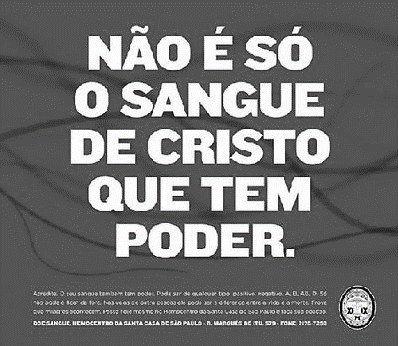
\includegraphics[width=3.03125in,height=2.63521in]{./imgSAEB_8_POR/media/image36.png}
\caption{Texto Descrição gerada automaticamente}
\end{figure}

\fonte{Disponível em: \url{http://www.diaadiaeducacao.pr.gov.br/portals/cadernospde/pdebusca/producoes\pde/2016/2016\pdp\port\uel\eldamariadeoliveiraesilva.pdf}
Acesso em: 21 fev. 2023.}

A campanha de doação de sangue remete ao texto bíblico com o objetivo de

\begin{escolha}
\item sensibilizar as pessoas com a lembrança da morte e ressurreição de
Cristo.
\item expressar religiosidade e divulgar a mensagem de Cristo para a
sociedade.
\item valorizar o doador, que com seu sangue pode salvar a vida de outra
pessoa.
\item restringir o público doador, que para doar precisa ser membro de uma
igreja.
\end{escolha}

\num{12}

\begin{quote}
Biosfera. O conjunto de todos os ecossistemas terrestres é chamado de
biosfera, que significa a camada de vida que envolve a Terra. É a área
do nosso planeta em que é possível a sobrevivência dos organismos vivos,
devido à existência de diversas condições que permitem a sustentação da
vida. Compreende não só a superfície terrestre, mas também uma parte da
atmosfera, do meio aquático e do subsolo. Tem aproximadamente 18
quilômetros, sendo 7 quilômetros para cima da superfície, na atmosfera,
e 11 quilômetros para baixo, até as profundezas marinhas. A biosfera
pode ser considerada o maior dos ecossistemas conhecidos.
\end{quote}

\fonte{RIOS, E.P.; THOMPSON, Miguel. \emph{Biomas brasileiros}. São Paulo:
Melhoramentos, 2013 (fragmento).}

Em razão das características do gênero, emprega-se no texto uma
linguagem que preza pelo(a)

\begin{escolha}
\item criatividade e autenticidade, com o objetivo de demarcar a autoria.

\item sentido literal das palavras, de modo a restringir a interpretação
das informações.

\item alternância da objetividade e da subjetividade, quando a opinião do
autor aparece.

\item sequenciação dos fatos no tempo e no espaço, a qual leva a um
desfecho inevitável.
\end{escolha}


\textbf{Texto para as questões 13 e 14.}

\begin{quote}
Merecer é um verbo que vem sendo muito utilizado ultimamente. Todo mundo
acha que merece uma porção de coisas. Tem gente que compra roupa nova
toda semana. Tem aqueles que adquirem relógios, computadores e outros
bens de consumo disponíveis no mercado.

Conheço mães que presenteiam seus filhos pequenos com brinquedos novos
num curto espaço de tempo, sem qualquer critério. Vejo homens que
costumam trocar de carro todos os anos e assim por diante.

Essas aquisições são feitas sob a desculpa do ``eu mereço''. E cada um
tem seus motivos para justificar esse merecimento. No entanto, muitas
vezes o tempo passa e as pessoas continuam extasiadas com seus pequenos
prazeres cotidianos, sem perceber que se contentam, na verdade, com
muito pouco.
\end{quote}

\fonte{DOMINGOS, Reinaldo. \emph{Como reduzir o impulso de comprar}. São Paulo:
DSOP Educação Financeira, 2013 (fragmento).}

\num{13}

Em seu texto, o autor desenvolve uma crítica ao comportamento

\begin{escolha}
\item egoísta, representado na fala ``eu mereço''.

\item consumista, justificado pela lei da compensação.

\item materialista, percebido no apego aos bens de consumo.

\item conformista, manifestado no contentamento com o pouco.
\end{escolha}

\num{14}

A finalidade comunicativa do texto indica que foi organizado em forma de

\begin{escolha}
\item relato pessoal.

\item nota de repúdio.

\item artigo de opinião.

\item carta de reclamação.
\end{escolha}


\num{15}

\textbf{TEXTO I}

\begin{quote}
\textbf{Com redução de crimes e outras ocorrências, Governo de Minas
promove o Carnaval mais seguro do Brasil}

\emph{Atuação conjunta das secretarias e planejamento estratégico das
forças de segurança garantiram sucesso da folia no estado}
\end{quote}

\fonte{AGÊNCIA MINAS, 23 fev. 2023. Disponível em:
\url{https://www.agenciaminas.mg.gov.br/noticia/com-reducao-de-crimes-e-outras-ocorrencias-governo-de-minas-promove-o-carnaval-mais-seguro-do-brasil.}
Acesso em: 04 mar. 2023 (fragmento).}

\textbf{TEXTO II}

\begin{quote}
\textbf{Carnaval de Minas Gerais registra queda expressiva de
criminalidade;}

\textbf{veja números}

\emph{Os dados são em comparação ao último Carnaval, em 2020, e mostram
queda de assaltos, furtos e importunação sexual}
\end{quote}

\fonte{CAVALCANTI, M. \emph{Rádio Itatiaia,} 23 fev. 2023. Disponível em:
\url{https://www.itatiaia.com.br/editorias/cidades/2023/02/23/carnaval-de-minas-gerais-registra-queda-expressiva-de-criminalidade-veja-numeros}.
Acesso em: 04 mar. 2023 (fragmento).}

Considerando-se as características do gênero textual, a diferença entre
os textos I e II se verifica

\begin{escolha}
\item na apresentação das informações fundamentais, tais como ``o quê'',
``quando'', ``quem'' e ``onde''.

\item na especificação dos tipos de crimes que foram cometidos e de
ocorrências que foram registradas.

\item nas marcas de parcialidade e imparcialidade com que se referem à
queda na criminalidade.

\item na veracidade das informações divulgadas, o que levanta dúvidas sobre
a credibilidade de um dos veículos.
\end{escolha}

\_\_\_\_\_\_\_\_\_\_\_\_\_\_\_\_\_\_\_\_\_\_\_\_\_\_\_\_\_\_\_\_\_\_\_\_\_\_\_\_\_\_\_\_\_\_\_\_\_\_\_\_\_\_\_\_\_\_\_\_\_\_\_\_\_\_\_\_\_\_\_\_\_

\section{Simulado 3}

\num{1}

\textbf{TEXTO I}

\begin{figure}
\centering
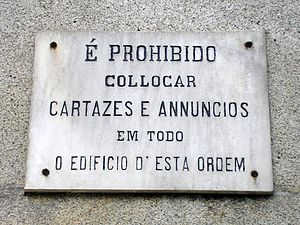
\includegraphics[width=2.21875in,height=1.66591in]{./imgSAEB_8_POR/media/image37.jpeg}
\caption{Texto Descrição gerada automaticamente}
\end{figure}

\fonte{
Disponível em: \url{https://commons.wikimedia.org/wiki/File:Placa\_pre-1911\_(Porto).jpg}. Acesso em: 27 fev. 2023.}

\textbf{TEXTO II}

\begin{longtable}[]{@{}l@{}}
\toprule
\endhead
\begin{minipage}[t]{0.30\columnwidth}\raggedright
É PROIBIDO

COLOCAR

CARTAZES E ANÚNCIOS

EM TODO

O EDIFÍCIO.\strut
\end{minipage}\tabularnewline
\bottomrule
\end{longtable}

\fonte{Elaborado pelo autor.}

O Texto II é uma reescrita do Texto I e ambos representam estágios
diferentes da língua portuguesa. Nesse sentido, exemplificam a variação
linguística

\begin{escolha}
\item
  social.
\item
  regional.
\item
  histórica.
\item
  situacional.
\end{escolha}

\num{2}

\begin{quote}
\textbf{A Raposa e as Uvas}

Uma Raposa, aproximando-se de uma parreira, viu que ela estava carregada
de uvas maduras e apetitosas. Com água na boca, desejou-as comer e, para
tanto, começou a fazer esforços para subir até elas. Porém, como
estivessem as uvas muito altas e fosse muito difícil a subida, a Raposa
tentou, mas não conseguiu alcançá-las. Disse então:

-- Estas uvas estão muito azedas e podem desbotar os meus dentes; não
quero colhê-las agora porque não gosto de uvas que não estão maduras.

E, dito isso, se foi.
\end{quote}

\fonte{Disponível em: \url{http://www.dominiopublico.gov.br/download/texto/ea000378.pdf}. Acesso em: 26 fev. 2023.}

No gênero narrativo fábula normalmente se pode reconhecer um ditado
popular que expressa um ensinamento. Essa fábula se relaciona com qual
ditado popular?

\begin{escolha}
\item Saco vazio não para em pé.

\item Quem tem pressa come cru.

\item Quem desdenha quer comprar.

\item Há males que vêm para o bem.
\end{escolha}

\num{3}

\begin{figure}
\centering
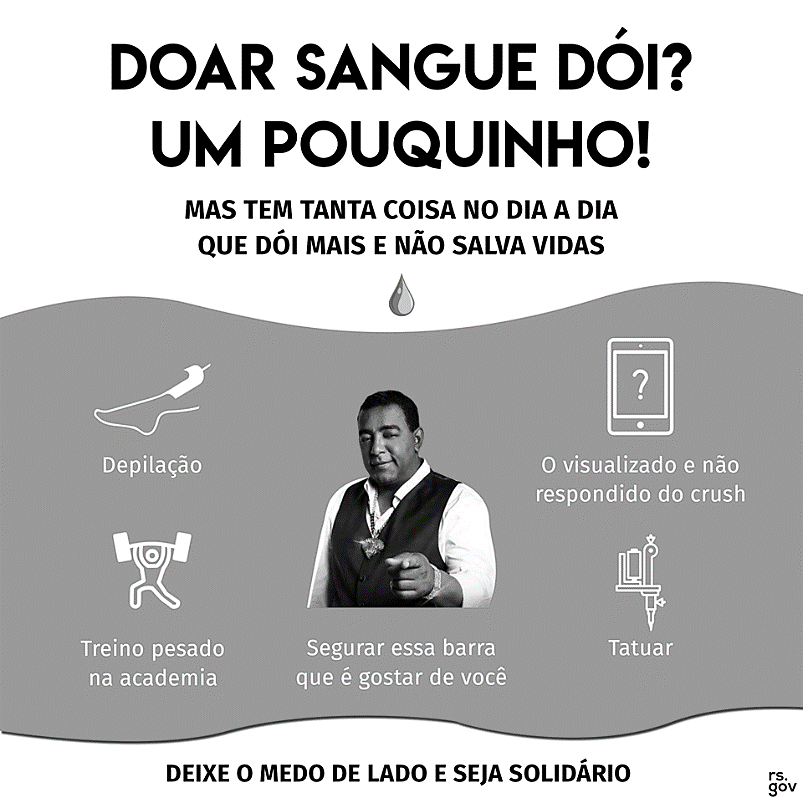
\includegraphics[width=3.65556in,height=3.65556in]{./imgSAEB_8_POR/media/image38.png}
\caption{Diagrama Descrição gerada automaticamente}
\end{figure}

\fonte{GOVERNO DO RIO GRANDE DO SUL. Disponível em: 
\url{https://www.facebook.com/GovernoDoRS/?locale=pt\BR}. Acesso em: 01 mar.
2023.}

O recurso persuasivo utilizado na campanha é o efeito de humor,
alcançado, sobretudo, por meio

\begin{escolha}
\item da relativização da dor.
\item da citação de uma canção.
\item da referência ao cotidiano.
\item da oposição medo-solidariedade.
\end{escolha}

\num{4}

\begin{quote}
A criança que fui chora na estrada.

Deixei-a ali quando vim ser quem sou.

Mas hoje, vendo que o que sou é nada,

Quero ir buscar quem fui onde ficou.
\end{quote}

\fonte{Fernando Pessoa.}

Em razão do gênero literário a que pertence, o texto caracteriza-se por
colocar em foco

\begin{escolha}
\item os sentimentos subjetivos do eu lírico.

\item a clareza e objetividade da mensagem.

\item a interpretação dramática de uma cena.

\item os elementos da sequência da narrativa.
\end{escolha}

\num{5}

Bula de Remédio: documento que acompanha um medicamento para orientar o
usuário quanto à ingestão.

A bula contém:

\begin{itemize}
\item
  Indicações;
\item
  Contraindicações;
\item
  Efeitos secundários;
\item
  Apresentação;
\item
  Fórmula ou composição;
\item
  Nome do laboratório;
\item
  Posologia (dose adequada).
\end{itemize}

\fonte{Elaborado pelo autor.}

O conteúdo da bula de remédio e sua finalidade comunicativa justificam,
na escrita desse gênero, o emprego de linguagem

\begin{escolha}
\item objetiva, para expor as informações do medicamento.

\item argumentativa, para dar uma opinião sobre o medicamento.

\item narrativa, para relatar as etapas de produção do medicamento.

\item figurada, para facilitar a compreensão dos dados do medicamento.
\end{escolha}


\textbf{Texto para as questões de 6 a 8.}

\begin{quote}
A história do futebol é uma triste viagem do prazer ao dever. {[}...{]}
O jogo se transformou em espetáculo, com poucos protagonistas e muitos
espectadores, futebol para olhar, e o espetáculo se transformou num dos
negócios mais lucrativos do mundo, que não é organizado para ser jogado,
mas para impedir que se jogue. A tecnocracia do esporte profissional foi
impondo um futebol de pura velocidade e muita força, que renuncia à
alegria, atrofia a fantasia e proíbe a ousadia. Por sorte ainda aparece
nos campos {[}...{]} algum atrevido que sai do roteiro e comete o
disparate de driblar o time adversário inteirinho, além do juiz e do
público das arquibancadas {[}...{]}.
\end{quote}

\fonte{GALEANO, E. \emph{Futebol ao sol e à sombra}. Porto Alegre: L\&PM, 1995
(fragmento).}

\num{6}

Nas relações de sentido construídas no texto, o termo ``dever'' se
relaciona, no contexto do futebol, com a ideia de roteiro, assim como
``prazer'' se relaciona com a ideia de

\begin{escolha}
\item improviso.

\item espetáculo.

\item velocidade.

\item tecnocracia.
\end{escolha}

\num{7}

Do ponto de vista do jogador, o futebol do dever e o futebol do prazer
caracterizam-se, respectivamente, por

\begin{escolha}
\item arte e criatividade.

\item velocidade e força.

\item monotonia e divertimento.

\item profissionalismo e várzea.
\end{escolha}

\num{8}

Para realçar as qualidades do futebol do prazer sobre as do futebol do
dever, o autor emprega exagero em

\begin{escolha}
\item ``o espetáculo se transformou num dos negócios mais lucrativos do
mundo.''

\item ``A tecnocracia do esporte profissional foi impondo um futebol de
pura velocidade e muita força.''

\item ``O jogo se transformou em espetáculo, com poucos protagonistas e
muitos espectadores.''

\item ``comete o disparate de driblar o time adversário inteirinho, além do
juiz e do público das arquibancadas.''
\end{escolha}

\num{9}

\begin{quote}
No Distrito Federal, uma reportagem revelou orientações ilegais contidas
em material utilizado no curso de formação de praças da PM. A Promotoria
Militar do Ministério Público do Distrito Federal e Territórios pediu
que a Corregedoria da Polícia Militar do DF abra investigação sobre a
denúncia, feita pelo colunista do UOL, Chico Alves.

Numa apresentação de PowerPoint sobre disciplina, ética, chefia e
liderança, conceitos teriam sido distorcidos para afirmar que, ao forjar
um flagrante ou praticar pequena tortura, o policial estaria agindo
corretamente.
\end{quote}

\fonte{Disponível em:
\url{https://agenciabrasil.ebc.com.br/direitos-humanos/noticia/2023-03/policia-militar-do-piaui-quer-formacao-antirracista-dos-agentes}.
Acesso em: 03 mar. 2023.}

Em se tratando do gênero notícia, a forma verbal ``teriam sido
distorcidos'' demonstra a intenção de

\begin{escolha}
\item reforçar a denúncia, pois a distorção dos conceitos ficou comprovada.

\item duvidar da veracidade do fato, pois a instituição denunciada é de
confiança.

\item atribuir a afirmação a um terceiro, pois a denúncia foi feita por
outro jornal.

\item amenizar a gravidade do fato, pois a distorção respeitou os limites
da lei.
\end{escolha}

\num{10}

\begin{quote}
VERA -- (sentando-se pensativa) Algo de ruim aconteceu a ele. Pode até
estar morto! Oh, Michael, estou tão angustiada com Dmitri.

MICHAEL -- Nunca vai amar outra pessoa além dele?

VERA -- (sorrindo) Não sei. Há muitas outras coisas para fazer no mundo
além de amar.

MICHAEL -- Nada mais vale a pena, Vera.

PETER -- Que barulho é este, Vera? (ouve-se um ruído metálico)

VERA -- (levantando-se e indo até a porta) Não sei, pai. Não se parece
com sinos de gado, senão poderia ser Nicholas retornando da feira.
\end{quote}

\fonte{WILDE, Oscar. \emph{Teatro completo}. Tradução de Doris Goettems. São
Paulo: Editora Landmark, 2011 (fragmento).}

O que caracteriza o texto como peça teatral é a presença de

\begin{escolha}
\item rubricas com instruções de interpretação da cena.

\item emoções subjetivas dos personagens, como a angústia.

\item indicações do tempo e espaço em que se passa a história.

\item discurso indireto em que as falas são reproduzidas pelo narrador.
\end{escolha}

\num{11}

\begin{quote}
Mito 04: ``Português é muito difícil'': os estudantes, principalmente,
utilizam essa afirmação (falsa!) para se referirem às\textbf{~}regras da
modalidade linguística aprendida na escola\textbf{,} e não ao uso real
que fazem do português. Afinal, eles se comunicam usando essa língua,
não é mesmo?
\end{quote}

\fonte{BAGNO, Marcos. \emph{Preconceito Linguístico}: o que é, como se faz.
Editora Parábola, 1999 (fragmento).}

O autor considera ser falsa a afirmação de que o português é uma língua
difícil. Para ele, o mito do português como língua difícil surgiu porque

\begin{escolha}
\item a escola ensina a gramática da língua de forma errada para os
estudantes.

\item os estudantes não se dedicam ao estudo da língua para aprenderem a
gramática.

\item a língua do cotidiano não tem regras, ao contrário da língua ensinada
na escola.

\item as pessoas pensam que a língua se limita às regras gramaticais
ensinadas na escola.
\end{escolha}

\num{12}

\begin{quote}
A gente se acostuma a morar em apartamentos de fundos e a não ter outra
vista que não as janelas ao redor. E, porque não tem vista, logo se
acostuma a não olhar para fora. E, porque não olha para fora, logo se
acostuma a não abrir de todo as cortinas. E, porque não abre as
cortinas, logo se acostuma a acender mais cedo a luz. {[}...{]}
\end{quote}

\fonte{COLASANTI, Marina. \emph{Eu sei, mas não devia}. Rio de Janeiro: Rocco,
1996 (fragmento).}

A repetição de certas palavras no texto contribui para a progressão
textual ao

\begin{escolha}
\item narrar a rotina da autora, do começo ao fim do dia.

\item justificar a preferência da autora por morar numa casa.

\item descrever ações realizadas, na ordem em que ocorreram.

\item enumerar situações que são consequências umas das outras.
\end{escolha}

\num{13}

\begin{quote}
TÍTULO I

Dos Princípios Fundamentais

Art. 1º A República Federativa do Brasil, formada pela união
indissolúvel dos Estados e Municípios e do Distrito Federal,
constitui-se em Estado Democrático de Direito e tem como fundamentos:

I - a soberania;

II - a cidadania;

{[}...{]}

Art. 2º São Poderes da União, independentes e harmônicos entre si, o
Legislativo, o Executivo e o Judiciário.

Art. 3º Constituem objetivos fundamentais da República Federativa do
Brasil:

I - construir uma sociedade livre, justa e solidária;

II - garantir o desenvolvimento nacional;

{[}...{]}
\end{quote}
\fonte{
Disponível em: \url{https://www.planalto.gov.br/ccivil\_03/constituicao/constituicaocompilado.htm}.
Acesso em: 03 mar. 2023.}

O texto de lei apresenta uma organização textual própria. O trecho
transcrito da Constituição é exemplar do gênero lei, pois

\begin{escolha}
\item determina as obrigações a serem cumpridas pelos cidadãos.

\item apresenta um vocabulário conhecido apenas por advogados.

\item estrutura os assuntos em artigos, elemento básico do gênero.

\item narra a evolução do país até se tornar uma república federativa.
\end{escolha}

\textbf{Texto para as questões 14 e 15.}

\begin{quote}
Vivia longe dos homens, só se dava bem com animais. Os seus pés duros
quebravam espinhos e não sentiam a quentura da terra. Montado,
confundia-se com o cavalo, grudava-se a ele. E falava uma linguagem
cantada, monossilábica e gutural, que o companheiro entendia. A pé, não
se aguentava bem. Pendia para um lado, para o outro lado, cambaio, torto
e feio. Às vezes, utilizava nas relações com as pessoas a mesma língua
com que se dirigia aos brutos -- exclamações, onomatopeias. Na verdade
falava pouco. Admirava as palavras compridas e difíceis da gente da
cidade, tentava reproduzir algumas em vão, mas sabia que elas eram
inúteis e talvez perigosas.
\end{quote}

\fonte{RAMOS, Graciliano. \textit{Vidas secas}. Rio de Janeiro: Record, 2013
(fragmento).}

\num{14}

A descrição física e psicológica do personagem contribui caracterizá-lo
como alguém

\begin{escolha}
\item tolo.

\item rústico.

\item analfabeto.

\item mal-humorado.
\end{escolha}

\num{15}

Em ``Na verdade falava pouco'', o narrador introduz uma

\begin{escolha}
\item conclusão.

\item reformulação.

\item exemplificação.

\item particularização.
\end{escolha}

\_\_\_\_\_\_\_\_\_\_\_\_\_\_\_\_\_\_\_\_\_\_\_\_\_\_\_\_\_\_\_\_\_\_\_\_\_\_\_\_\_\_\_\_\_\_\_\_\_\_\_\_\_\_\_\_\_\_\_\_\_\_\_\_\_\_\_\_\_\_

\section{Simulado 4}

\num{1}

\begin{quote}
\textbf{Campus Party: reciclagem de lixo eletrônico dá origem a projetos
sociais}

A cada dia surgem novos modelos de computadores, smartphones, câmeras
digitais e outros diversos produtos eletrônicos. A velocidade dos
lançamentos e atualizações faz com que esses equipamentos se tornem
obsoletos rapidamente, e assim cresce a demanda por uma destinação
correta para o lixo eletrônico. Projetos que atuam na reutilização
desses objetos estão sendo apresentados na Campus Party Brasília, que é
realizada até este sábado (17).
\end{quote}

  \fonte{Disponível em:\url{https://agenciabrasil.ebc.com.br/pesquisa-e-inovacao/noticia/2017-06/campus-party-reciclagem-de-lixo-eletronico-da-origem-projetos}.
Acesso em: 08 mar. 2023 (fragmento).}

Da leitura do texto, depreende-se que a grande quantidade gerada de lixo
eletrônico tem como causa

\begin{escolha}
\item a obsolescência dos eletrônicos em razão das rápidas inovações
tecnológicas.

\item o descarte dos equipamentos eletrônicos de forma incorreta no meio
ambiente.

\item a qualidade baixa dos equipamentos eletrônicos que leva a uma curta
vida útil.

\item a falta de projetos sociais que possam dar uma destinação adequada
aos eletrônicos.
\end{escolha}

\num{2}

\begin{quote}
\textbf{Obesidade infantil é tema do programa Salto para o Futuro}

Um dos problemas de saúde pública mais preocupantes atualmente, a
obesidade infantil, será o tema da próxima edição do
programa~\emph{Salto para o Futuro}, nesta quarta-feira, 18, às 20h, na
TV Escola. A escolha da matéria não acontece por acaso, uma vez que a
Organização Mundial de Saúde (OMS), em seu estudo mais recente de
outubro de 2017, apontou um total de 124 milhões de crianças e
adolescentes obesos em todo o mundo.

{[}...{]}

As causas da doença e as medidas para evitar que crianças, adolescentes
e jovens se tornem obesos são o foco desta edição do programa da TV
Escola.
\end{quote}

\fonte{Disponível em:
\url{http://portal.mec.gov.br/ultimas-noticias/33491-tv-escola/63021-obesidade-infantil-e-tema-do-programa-salto-para-o-futuro}.
Acesso em: 08 mar. 2023 (fragmento adaptado).}

No último parágrafo, o termo ``doença'', além de retomar ``obesidade
infantil'', adiciona-lhe um valor semântico. Nesse sentido, o termo
retoma a expressão ``obesidade infantil'' e, ao mesmo tempo,

\begin{escolha}
\item situa-a no horizonte de preocupação da medicina como um problema de
saúde.

\item atenua a gravidade com que se deve observar a obesidade na juventude.

\item relaciona-a aos dados estatísticos da Organização Mundial de Saúde.

\item chama o espectador a acompanhar a edição do programa divulgado.
\end{escolha}

\num{3}

\textbf{TEXTO I}

\begin{quote}
\textbf{Organização e segurança são destaques no carnaval de rua de São
Paulo}

\emph{Prévia de pesquisa entre os foliões de ruas aponta que a
organização teve aprovação de 96,3\% com nota de 8,8, em escala de zero
a dez. Já para o público que esteve no sambódromo, a nota final foi 9
(mais de 50\% deram 10)}
\end{quote}

\fonte{SECRETARIA ESPECIAL DE COMUNICAÇÃO, 23 fev. 2023. Disponível em:
capital.sp.gov.br/noticia/organizacao-e-seguranca-sao-destaques-no-carnaval-de-rua-de-sao-paulo.
Acesso em: 04 mar. 2023.}

\textbf{TEXTO II}

\begin{quote}
\textbf{Mais de 3 mil celulares foram furtados durante o carnaval em SP}

\emph{Número é quase 40\% inferior aos registrados de 2020}

Durante o período de carnaval foram registrados 3.486 roubos e furtos de
celulares no estado de São Paulo, segundo balanço divulgado hoje (22)
pela Secretaria de Segurança Pública de São Paulo.

O número é quase 40\% inferior à quantidade de registros de roubos e
furtos ocorridos no carnaval de 2020, quando foram feitos 5.450 boletins
de ocorrência. O número também é inferior ao que foi registrado no
carnaval de 2019, quando foram lavrados 5.471 boletins.
\end{quote}

\fonte{AGÊNCIA BRASIL, 22 fev. 2023. Disponível em:
\url{https://agenciabrasil.ebc.com.br/geral/noticia/2023-02/mais-de-3-mil-celulares-foram-furtados-durante-o-carnaval-em-sp}.
Acesso em: 04 mar. 2023.}

A aparente divergência entre as informações apresentadas nessas notícias
é afastada

\begin{escolha}
\item pelo conhecimento prévio do leitor.

\item pela presença de dados estatísticos.

\item pela credibilidade dos veículos.

\item pelo meio de circulação.
\end{escolha}

\textbf{Texto para as questões 4 e 5.}

\begin{figure}
\centering
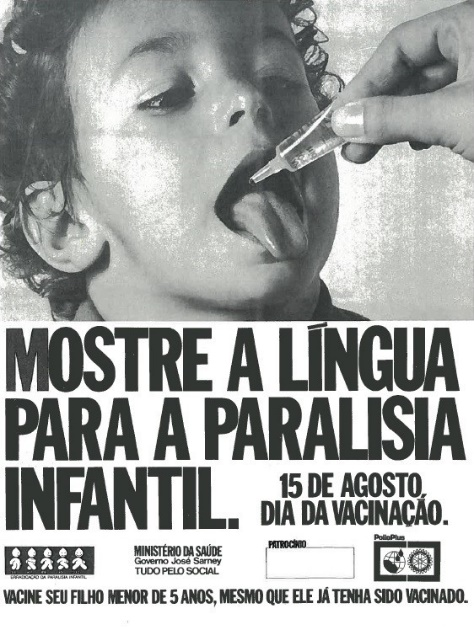
\includegraphics[width=2.12879in,height=2.83333in]{./imgSAEB_8_POR/media/image39.jpeg}
\caption{Texto Descrição gerada automaticamente}
\end{figure}

\fonte{Disponível em: \url{https://bvsms.saude.gov.br/bvs/folder/10006001944.pdf}.
Acesso em: 09 mar. 2023 (adaptado).}

\num{4}

A campanha, na linguagem verbal e não verbal, busca ganhar a adesão do
público por meio da ênfase

\begin{escolha}
\item na data da vacinação.

\item no motivo da vacinação.

\item no método de vacinação.

\item no público da vacinação.
\end{escolha}


\num{5}

Textos publicitários utilizam diferentes recursos na construção da
mensagem. Na campanha apresentada, o recurso utilizado é

\begin{escolha}
\item
a imparcialidade, para evitar influenciar a adesão do público.
\item
o efeito humorístico, gerado pela pose da criança na fotografia.
\item
a duplicidade de sentidos, como na expressão ``mostre a língua''.
\item
a linguagem literal, privilegiando o sentido denotativo das palavras.
\end{escolha}

\num{6}

\begin{quote}
Passava das 11 horas da noite quando Bento deixou a fazendo do compadre
Chico em sua velha caminhonete vermelha. Estava a pouco menos de vinte
quilômetros de sua casa. Conhecia o caminho como a palma da mão. Os
primeiros cinco quilômetros eram asfaltados. O resto parecia uma
montanha-russa de terra batida, repleta de pedregulhos. Ao passar pela
última porteira, ligou o rádio. Acordara às 6 da manhã e não queria
dormir ao volante. Perdera o melhor amigo em um acidente naquele mesmo
trajeto.
\end{quote}

\fonte{FARAH, F.T. \emph{O enigma das estrelas.} São Paulo: Geração Editorial,
2013 (fragmento).}

Há sentido figurado em

\begin{escolha}
\item ``Os primeiros cinco quilômetros eram asfaltados''.

\item ``O resto parecia uma montanha-russa de terra batida''.

\item ``Estava a pouco menos de vinte quilômetros de sua casa''.

\item ``Perdera o melhor amigo em um acidente naquele mesmo trajeto''.
\end{escolha}


\num{7}

\begin{quote}
Era uma O ônibus Greyhound fez sua parada regular em Meade, Ohio, uma
insignificante cidade produtora de papel a uma hora ao sul de Columbus
que cheirava a ovo podre. Forasteiros

reclamavam do fedor, mas os moradores gostavam de se vangloriar de que
aquele era o doce aroma do dinheiro. O motorista, um homem simplório e
atarracado que usava sapatos com salto e uma gravata borboleta frouxa,
parou no beco ao lado da estação e anunciou uma parada de quarenta
minutos. Desejava poder tomar uma xícara de café, porém sua úlcera
estava atacando novamente. Bocejou e deu um gole numa garrafa de um
remédio rosa que deixava no painel. A chaminé do outro lado da cidade,
de longe a estrutura mais alta naquela parte do estado, arrotava mais
uma nuvem marrom e suja. Era possível vê-la por quilômetros, soprando
como um vulcão prestes a estourar seu topo estreito.
{[}...{]}
\end{quote}

\fonte{POLLOCK, Donald Ray. \emph{O mal nosso de cada dia}. Tradução de Paulo
Raviere. Rio de Janeiro: DarkSide Books, 2020.}

Pelo conteúdo do texto, e sabendo que se trata de uma narrativa, pode-se
reconhecer que esse parágrafo apresenta

\begin{escolha}
\item o desfecho, que introduz a resolução do problema surgido na história.

\item o conflito, que introduz o problema que precisa ser resolvido na
história.

\item a situação inicial, que introduz o tempo, o espaço e os personagens
da história.

\item o clímax, que introduz as tensões entre os personagens e reviravoltas
na história.
\end{escolha}

\textbf{Texto para as questões 8 e 9.}

\begin{quote}
Uma noite destas, vindo da cidade para o Engenho Novo, encontrei no trem
da Central um rapaz aqui do bairro, que eu conheço de vista e de chapéu.
Cumprimentou-me, sentou-se ao pé de mim, falou da Lua e dos ministros, e
acabou recitando-me versos. A viagem era curta, e os versos pode ser que
não fossem inteiramente maus. Sucedeu, porém, que, como eu estava
cansado, fechei os olhos três ou quatro vezes; tanto bastou para que ele
interrompesse a leitura e metesse os versos no bolso.

--- Continue, disse eu acordando.

--- Já acabei, murmurou ele.

--- São muito bonitos.

Vi-lhe fazer um gesto para tirá-los outra vez do bolso, mas não passou
do gesto; estava amuado. No dia seguinte entrou a dizer de mim nomes
feios, e acabou alcunhando-me Dom Casmurro. Os vizinhos, que não gostam
dos meus hábitos reclusos e calados, deram curso à alcunha, que afinal
pegou. Nem por isso me zanguei. Contei a anedota aos amigos da cidade, e
eles, por graça, chamam-me assim, alguns em bilhetes: ``Dom Casmurro,
domingo vou jantar com você''. {[}...{]}
\end{quote}

\fonte{ASSIS, Machado de.~\emph{Dom Casmurro}.~Rio de Janeiro: Nova Aguilar,
1994 (fragmento).}

\num{8}

O narrador considera ser uma anedota a situação que vivenciou com um
rapaz no trem. A situação pode ser considerada engraçada porque

\begin{escolha}
\item a conversa entre o narrador e o rapaz abordou diferentes assuntos.

\item o rapaz interrompeu a leitura e guardou os versos do poema no bolso.

\item o narrador evitou dar atenção ao rapaz por conhecê-lo apenas de
vista.

\item o cansaço do narrador foi confundido com falta de interesse no poema.
\end{escolha}

\num{9}

De acordo com o contexto, o uso da expressão ``fechei os olhos três ou
quatro vezes'' teve o objetivo de

\begin{escolha}
\item diminuir a importância do motivo causador da indignação do rapaz.

\item concordar com o motivo de o rapaz ter desistido da leitura dos
versos.

\item indicar a quantidade de vezes que dormiu ao longo da conversa.

\item justificar sua indiferença em relação ao poema lido pelo rapaz.
\end{escolha}

\num{10}

\begin{quote}
\textbf{O goleiro}

Também chamado de porteiro, guarda-metas, arqueiro, guardião, golquíper
ou guarda-valas, mas poderia muito bem ser chamado de mártir, vítima,
saco de pancadas, eterno penitente ou favorito das bofetadas. Dizem que
onde ele pisa, nunca mais cresce a grama. {[}...{]}

Os outros jogadores podem errar feio uma vez, muitas vezes, mas se
redimem com um drible espetacular, um passe magistral, um tiro certeiro.
Ele, não. A multidão não perdoa o goleiro. Saiu em falso? Catando
borboleta? Deixou a bola escapar? Os dedos de aço se fizeram de seda?
Com uma só falha, o goleiro arruína uma partida ou perde um campeonato,
e então o público esquece subitamente todas as suas façanhas e o condena
à desgraça eterna. Até o fim de seus dias, será perseguido pela
maldição.
\end{quote}

\fonte{GALEANO, Eduardo. \emph{Futebol ao sol e à sombra}. Tradução de Eric
Nepomuceno e Maria do Carmo Brito. Porto Alegre: L\&PM Pocket, 2014
(fragmento).}

O texto aborda a profissão de goleiro com tom humorístico. O efeito de
humor se manifesta por meio de

\begin{escolha}
\item caracterização pejorativa e exagero.

\item uso de termos e expressões ofensivos.

\item desqualificação das habilidades do goleiro.

\item exaltação dos jogadores de linha.
\end{escolha}

\num{11}

\begin{quote}\textbf{Manutenção}

Aumente a vida útil do aparelho, limpe-o regularmente!

NOTA: Antes de iniciar a limpeza do equipamento desligue-o da tomada.

\textbf{Limpando a tela}

\num{1} Molhe um pano macio em uma mistura de água morna com um pouco de
detergente. Esprema bem o pano até que ele fique quase seco e então
utilize-o em sua tela.

\num{2} Para garantir que não exista resíduos líquidos na tela, deixe-a
secar por alguns minutos e só depois ligue o aparelho na tomada.
\end{quote}

\fonte{Disponível em:
\url{https://www.lg.com/br/products/documents/MFL59166617\_BBTV\_SERIES\_REV00.pdf}.
Acesso em: 10 mar. 2023 (fragmento).}

Devido ao gênero a que pertence, o texto apresenta, em sua composição,
verbos no imperativo que expressam o sentido de

\begin{escolha}
\item comando, para que o usuário se sinta obrigado a limpar o equipamento.

\item recomendação, para que o usuário faça a correta limpeza do
equipamento.

\item apelo, para que o usuário reconheça a necessidade de limpar o
equipamento.

\item convite, para que o leitor seja convencido a realizar a limpeza do
equipamento.
\end{escolha}

\num{12}

\textbf{TEXTO I}

\begin{quote}

\textbf{Isto}

Dizem que finjo ou minto

Tudo que escrevo. Não.

Eu simplesmente sinto

Com a imaginação.

Não uso o coração.

Tudo o que sonho ou passo,

O que me falha ou finda,

É como que um terraço

Sobre outra coisa ainda.

Essa coisa é que é linda.

Por isso escrevo em meio

Do que não está ao pé,

Livre do meu enleio,

Sério do que não é.

Sentir? Sinta quem lê!
\end{quote}

\fonte{PESSOA, Fernando. Disponível em:
\url{http://arquivopessoa.net/typographia/textos/arquivopessoa-4250.pdf}.
Acesso em: 10 mar. 2023.}

\textbf{TEXTO II}

\begin{quote}
\textbf{Autopsicografia}

O poeta é um fingidor

Finge tão completamente

Que chega a fingir que é dor

A dor que deveras sente.

E os que leem o que escreve,

Na dor lida sentem bem,

Não as duas que ele teve,

Mas só a que eles não têm.

E assim nas calhas de roda

Gira, a entreter a razão,

Esse comboio de corda

Que se chama coração.
\end{quote}

\fonte{PESSOA, Fernando. Disponível em: \url{http://arquivopessoa.net/textos/4234}. Acesso em: 10 mar. 2023.}

Os dois poemas se relacionam intertextualmente por

\begin{escolha}
\item pertencerem ao mesmo autor.

\item concordarem no mesmo ponto de vista.

\item abordarem o mesmo tema: o fazer poético.

\item apresentarem a mesma estrutura de estrofes.
\end{escolha}

\num{13}

\begin{quote}
\textbf{Como nuvens pelo céu}

Como nuvens pelo céu

Passam os sonhos por mim.

Nenhum dos sonhos é meu

Embora eu os sonhe assim.

São coisas no alto que são

Enquanto a vista as conhece,

Depois são sombras que vão

Pelo campo que arrefece.

Símbolos? Sonhos? Quem torna

Meu coração ao que foi?

Que dor de mim me transtorna?

Que coisa inútil me dói?
\end{quote}

\fonte{PESSOA, Fernando. Disponível em: \url{http://arquivopessoa.net/textos/1063}.
Acesso em: 13 mar. 2023.}

O eu lírico utiliza, em sua reflexão, uma comparação com as nuvens por
sua característica de serem

\begin{escolha}
\item lúdicas.

\item uniformes.

\item transitórias.

\item reconhecíveis.
\end{escolha}

\num{14}

\begin{quote}
Assim como acontece em várias famílias brasileiras, na minha há uma
prática comum: quem ascende socialmente numa capital (no caso, Salvador)
acaba ``puxando'' os parentes do interior. No meu lado paterno, quem
cumpriu esse papel foi Dindinha, tia-avó de meu pai. Ela, aliás, levou
esse costume ao extremo: recebemos nada menos que dezenove sobrinhos na
sua casa, no bairro da Federação.
\end{quote}

\fonte{RAMOS, Lázaro. \emph{Na minha pele}. 1.ed. Rio de Janeiro: Objetiva,
2017 (fragmento).}

Os termos ``esse papel'' e ``esse costume'' contribuem para a progressão
textual ao evitarem repetição de palavras e

\begin{escolha}
\item provocarem mudança de assunto.

\item fazerem referência externa ao texto.

\item anteciparem o que ainda vai ser dito.

\item retomarem o mesmo trecho antecedente.
\end{escolha}

\num{15}

\begin{quote}
Se eu pudesse trincar a terra toda

E sentir-lhe um paladar,

Seria mais feliz um momento...

Mas eu nem sempre quero ser feliz.

É preciso ser de vez em quando infeliz

Para se poder ser natural...

Nem tudo é dias de sol,

E a chuva, quando falta muito, pede-se.

Por isso tomo a infelicidade com a felicidade

Naturalmente, como quem não estranha

Que haja montanhas e planícies

E que haja rochedos e erva...

O que é preciso é ser-se natural e calmo

Na felicidade ou na infelicidade,

Sentir como quem olha,

Pensar como quem anda,

E quando se vai morrer, lembrar-se de que o dia morre,

E que o poente é belo e é bela a noite que fica...

Assim é e assim seja...
\end{quote}

\fonte{PESSOA, Fernando. Disponível em: \url{http://arquivopessoa.net/textos/613}.
Acesso em: 19 mar. 2023.}

O verso final do poema, ``Assim é e assim seja...'', confirma a visão de
mundo exposta ao longo do texto. O eu poético, nesse verso, assume, em
relação aos infortúnios da vida, uma postura de

\begin{escolha}
\item conformismo

\item negação.

\item pessimismo.

\item indignação.
\end{escolha}

\section{Referências}

ALMEIDA, L. de. \textbf{Análise semântica de operadores argumentativos
em textos publicitários}. 2001. 187 f.~Dissertação (Mestrado em Estudos
Linguísticos). Programa de PósGraduação em Estudos Linguísticos,
Instituto de Letras e Linguística, Universidade Federal de Uberlândia,
2001.

CEGALLA, Domingos Paschoal. \textbf{Novíssima gramática da língua
portuguesa}. 48. ed.~São Paulo: IBEP, 2009.

CHALHUB, Samira. \textbf{Funções da linguagem}. 11 ed.~São Paulo: Ática,
2000.

MARCUSCHI, Luiz Antônio. Gêneros textuais: definição e funcionalidade.
In: DIONISIO, Angela Paiva; MACHADO, Anna Rachel; BEZERRA, Maria
Auxiliadora (Org.). \textbf{Gêneros textuais \& ensino}. São Paulo:
Parábola, 2010. p.~23.

PORSCHE, Sandra Cristina. et al.~\textbf{O gênero verbete no ensino}.
Simpósio Internacional de Gêneros Textuais. Disponível em:
\textless{}\url{https://www.ucs.br/ucs/extensao/agenda/eventos/vsiget/portugues/anais/arquivos/o_genero_verbete_no_ensino.pdf}\textgreater.
Acessado em: 03/07/2018.

SARMENTO, Leila Luar: TUFANO: Douglas.~\textbf{Literatura, Gramática e
Produção de Texto}. São Paulo: Moderna, 2001.
